\chapter{Evaluation}\label{chapter:evaluation}
In this chapter, we evaluate the performance of our prototype regular expressions engine compared to other popular C++ regular expressions engines. The benchmarks were run on a server with a twenty-core Intel(R) Core(TM) i9-7900X @ 3.30GHz processor, 128 GiB RAM running Ubuntu 21.10.

The code for generating and running benchmarks, as well as raw run results, are available in our repository on Github \footnote{\url{https://github.com/melzareix/jit-regex}}.

\newcounter{magicrownumbers1}
\newcounter{magicrownumbers2}
\newcounter{magicrownumbers3}
\newcommand\rownumberone{\stepcounter{magicrownumbers1}\arabic{magicrownumbers1}}
\newcommand\rownumbertwo{\stepcounter{magicrownumbers2}\arabic{magicrownumbers2}}
\newcommand\rownumberthree{\stepcounter{magicrownumbers3}\arabic{magicrownumbers3}}

\section{DFA Compilation Time Evaluation}
In this section, we evaluate the compilation time for the two backends \textbf{\{LLVM, CPP\}} and the two Unicode encoding mechanisms \textbf{\{UTF-8, UTF-32\}}.

Benchmarking the compilation time aims to:
\begin{enumerate}
    \item Test our assumption that LLVM compilation is faster than C++ for our use case. Moreover, if our assumptions are correct, how much speedup do we get when using LLVM compared to C++?
    \item Compare the effect on compilation time performance using different UTF encoding mechanisms.
\end{enumerate}

In the following benchmarks, for each backend and encoding mechanism, we pass a text file containing a list of regular expressions. Each backend reads the file line by line, compiles each pattern to a DFA, and generates code that matches the pattern. It finally passes the code to the LLVM JIT compiler to get a function pointer that can be used to match the pattern.

\subsection{Common Patterns Benchmark}\label{cmnpatt}
RegExLib \cite{regexlib} is a popular Regular Expressions repository on the Web, with expressions for matching URIs, HTML code, C-style strings, Java code, SQL queries, spam, etc. We extracted ten top rated patterns (Table \ref{tab:cmpbench}) from RegExLib to use in this benchmark.

{\renewcommand{\arraystretch}{1.5}% for the vertical padding
\begin{table}[H]
\centering
\small
\begin{tabularx}{\textwidth}{|l|X|}
\hline
\# & Pattern       \\
\hline
\rownumbertwo & \texttt{\textbf{{[}a-zA-Z0-9 {]}*}}\\ \hline
\rownumbertwo & \texttt{\textbf{{[}2-9{]}{[}0-9{]}\{2\}-{[}0-9{]}\{3\}-{[}0-9{]}\{4\}}}\\ \hline
\rownumbertwo & \texttt{\textbf{{[}a-zA-Z0-9.\_\%-{]}+@{[}a-zA-Z0-9.-{]}+.{[}a-zA-Z{]}\{2,6\}}}\\ \hline
\rownumbertwo & \texttt{\textbf{{[}0-9{]}*.?{[}0-9{]}*}}\\ \hline
\rownumbertwo & \texttt{\textbf{({[}0-1{]}{[}0-9{]}|{[}2{]}{[}0-3{]}):({[}0-5{]}{[}0-9{]})}}\\ \hline
\rownumbertwo & \texttt{\textbf{({[}0-9{]}\{3\})?|({[}0-9{]}\{3\})({[}-./{]}?)({[}0-9{]}\{3\})({[}0-9-./{]}?)({[}0-9{]}\{4\})}}\\ \hline
\rownumbertwo & \texttt{\textbf{{[}-+{]}?{[}0-9{]}+{[}.{]}?{[}0-9{]}*({[}eE{]}{[}-+{]}?{[}0-9{]}+)?}}\\ \hline
\rownumbertwo & \texttt{\textbf{({[}0-9{]}\{1,2\}|1{[}0-9{]}{[}0-9{]}|2{[}0-4{]}{[}0-9{]}|25{[}0-5{]})({[}0-9{]}\{1,2\}|1{[}0-9{]}{[}0-9{]}|2{[}0-4{]}{[}0-9{]}|25{[}0-5{]})({[}0-9{]}\{1,2\}|1{[}0-9{]}{[}0-9{]}|2{[}0-4{]}{[}0-9{]}|25{[}0-5{]})({[}0-9{]}\{1,2\}|1{[}0-9{]}{[}0-9{]}|2{[}0-4{]}{[}0-9{]}|25{[}0-5{]}) }}\\ \hline
\rownumbertwo & \texttt{\textbf{{[}a-zA-Z0-9@*\#{]}\{8,15\}}}\\ \hline
\rownumbertwo & \texttt{\textbf{{[}0-9{]}\{1,3\}(,{[}0-9{]}\{3\})*|({[}0-9{]}+)(.{[}0-9{]}\{2\})?}}\\
\hline

\end{tabularx}
\caption{Patterns in the Common Patterns Benchmark. When compiling all the patterns are prefixed with \texttt{\textbf{\%}} meta-character to find partial matches.}\label{tab:cmpbench}
\end{table}}

Figure \ref{fig:eval_common} shows the results of the benchmark. The results confirm our assumption that the LLVM backend compilation is faster than C++ code regardless of the Unicode encoding mechanism ($9x$ speedup). This speedup can be explained by the fact that when generating LLVM code, everything is done in memory, and no CPU time is wasted. While for C++, we have to write the code to the disk, wait for the \texttt{clang} compiler to execute then read the generated IR again before JITing.

The results also show that for this benchmark, UTF-32 encoding is slightly faster than UTF-8, achieving a speedup of $1.2x$. This speedup is attributed to the patterns being small in size and number, and the patterns are non-Unicode, so UTF-32 generates smaller automata and does not take extra time to process the pattern code points.

\begin{figure}[H]
\hspace*{-45pt}

\centering
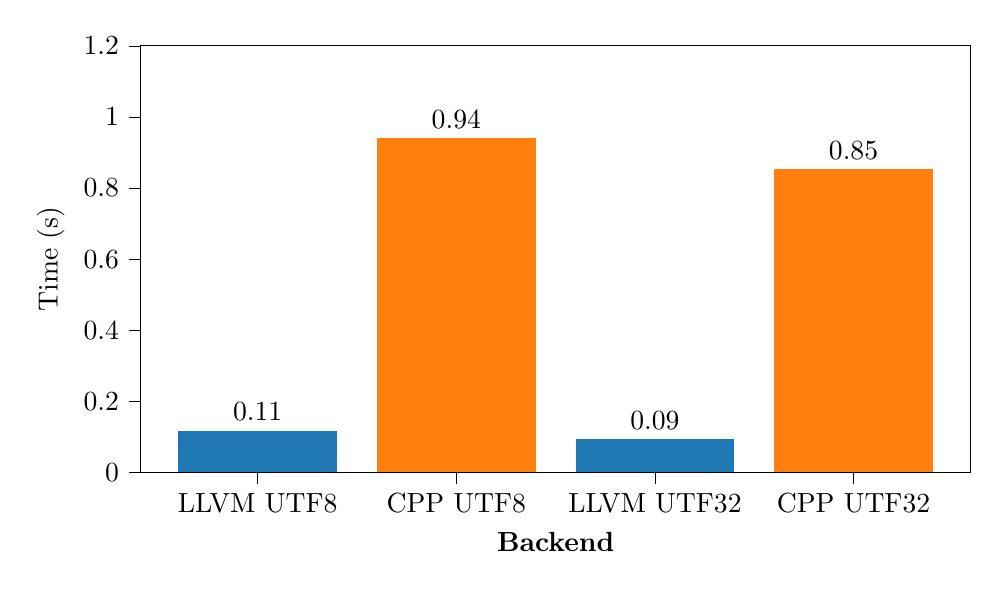
\begin{tikzpicture}
\definecolor{darkgray176}{RGB}{176,176,176}
\definecolor{darkorange25512714}{RGB}{255,127,14}
\definecolor{steelblue31119180}{RGB}{31,119,180}
\begin{axis}[
% scale only axis,
width={\textwidth},
% height=\axisdefaultheight,
height=7cm,
tick align=outside,
tick pos=left,
x grid style={darkgray176},
xlabel={\textbf{Backend}},
xmin=-0.59, xmax=3.59,
xtick style={color=black},
xtick={0,1,2,3},
xticklabels={LLVM UTF8,CPP UTF8,LLVM UTF32,CPP UTF32},
y grid style={darkgray176},
ylabel={Time (s)},
ymin=0, ymax=1.2,
ytick style={color=black}
]
\draw[draw=none,fill=steelblue31119180] (axis cs:-0.4,0) rectangle (axis cs:0.4,0.11753389959534);
\draw[draw=none,fill=darkorange25512714] (axis cs:0.6,0) rectangle (axis cs:1.4,0.941184333836039);
\draw[draw=none,fill=steelblue31119180] (axis cs:1.6,0) rectangle (axis cs:2.4,0.0936958231031895);
\draw[draw=none,fill=darkorange25512714] (axis cs:2.6,0) rectangle (axis cs:3.4,0.852185526241859);


\draw (axis cs:0,0.11753389959534) ++(0pt,0pt) node[
      scale=1,
      anchor=south,
      text=black,
      rotate=0.0
    ]{0.11};

\draw (axis cs:1,0.941184333836039) ++(0pt,0pt) node[
      scale=1,
      anchor=south,
      text=black,
      rotate=0.0
    ]{0.94};

\draw (axis cs:2,0.0936958231031895) ++(0pt,0pt) node[
      scale=1,
      anchor=south,
      text=black,
      rotate=0.0
    ]{0.09};
    
\draw (axis cs:3,0.852185526241859) ++(0pt,0pt) node[
      scale=1,
      anchor=south,
      text=black,
      rotate=0.0
    ]{0.85};
    
\end{axis}


\end{tikzpicture}

\caption{Compilation time performance for the Common Patterns Benchmark. Benchmark was run three times and the mean ($\mu$) of the three runs is taken. Y-axis is the time (in seconds) taken by each backend to compile \textbf{all} patterns in the benchmark.}
\label{fig:eval_common}
\end{figure}

\subsection{GitHub SQL Benchmark}
The results from the previous benchmark in subsection \ref{cmnpatt} were promising and aligned with our assumptions. We created another benchmark to further test our assumptions by scraping $524$ regular expressions from open-source projects on GitHub. These projects were SQL projects, and patterns are SQL-flavored regular expressions. Seventy-seven of these patterns contain Unicode characters, which would showcase the performance of the engine on Unicode. Table \ref{tab:samplesql} shows a sample of these patterns.

{\renewcommand{\arraystretch}{1.2}% for the vertical padding
\begin{table}[H]
\centering
\small
\begin{tabularx}{\textwidth}{|l|X|}
\hline
\# & Pattern       \\
\hline
\rownumberone & \texttt{\textbf{{[}{[}:ALNUM:{]}.\_\%+-{]}+@{[}{[}:ALNUM:{]}.-{]}+.{[}{[}:ALPHA:{]}{]}+}} \\
\hline
\rownumberone & \texttt{\textbf{\${[}0-9{]}+(.{[}0-9{]}{[}0-9{]})?}}                                      \\
\hline
\rownumberone &\texttt{\textbf{\%AK Email Signup\%}}                                                     \\
\hline
\rownumberone &\texttt{\textbf{\%Assistant\%(I)*}}                                                       \\
\hline
\rownumberone &\texttt{\textbf{{[}A-Z{]}{[}0-9{]}\{3\}-{[}0{]}{[}A-Z{]}\{2\}}}                          \\
\hline
\rownumberone & \texttt{\textbf{\%(汉服|国创|国漫|国潮|姜子牙|哪吒|东方美|中国风)\%}}     \\            
\hline
\end{tabularx}
\caption{Sample of the patterns in the Github SQL Benchmark. When compiling all the patterns are prefixed with \texttt{\textbf{\%}} meta-character to find partial matches.}\label{tab:samplesql}
\end{table}}

Figure \ref{fig:eval_sql} shows the results of the benchmark. The results again show the compilation performance advantage of LLVM backends over C++ backends. LLVM backend compilation achieved a speedup of $\sim9x$ compared to C++ code for both encodings.

The results also show a performance advantage for UTF-8 over UTF-32 
with a speedup of $2x$ for the LLVM backend and $1.6x$ for the C++ backend, contrary to, the results from the common patterns benchmark. To further investigate the reason behind this, we removed the Unicode patterns from the benchmark and re-ran the benchmark.

The results after removing Unicode patterns were aligned with the first benchmark. UTF-32 encoding was $1.36x$ faster than UTF-8 for LLVM and $1.22x$ for C++ backend. The reason for this slowdown for UTF-32 on Unicode is that although UTF-32 generates smaller automata compared to UTF-8, it has to read and verify the whole Unicode code-point. This takes extra time and is slower than UTF-8 which only works with bytes at compilation.

\begin{figure}[H]
\centering
\hspace*{-45pt}
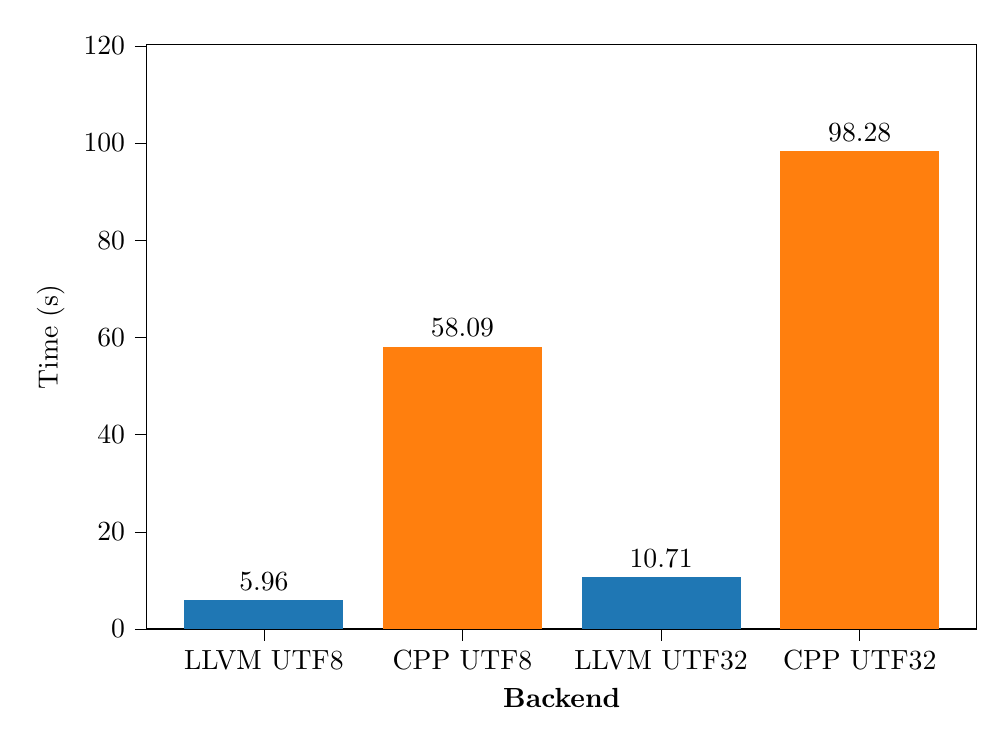
\begin{tikzpicture}

\definecolor{darkgray176}{RGB}{176,176,176}
\definecolor{darkorange25512714}{RGB}{255,127,14}
\definecolor{steelblue31119180}{RGB}{31,119,180}

\begin{axis}[
% scale only axis,
width={\textwidth},
height=9cm,
tick align=outside,
tick pos=left,
x grid style={darkgray176},
xlabel={\textbf{Backend}},
xmin=-0.59, xmax=3.59,
xtick style={color=black},
xtick={0,1,2,3},
xticklabels={LLVM UTF8,CPP UTF8,LLVM UTF32,CPP UTF32},
y grid style={darkgray176},
ylabel={Time (s)},
ymin=0, ymax=120.19825138282,
ytick style={color=black}
]
\draw[draw=none,fill=steelblue31119180] (axis cs:-0.4,0) rectangle (axis cs:0.4,5.96466026082635);
\draw[draw=none,fill=darkorange25512714] (axis cs:0.6,0) rectangle (axis cs:1.4,58.0985493951788);
\draw[draw=none,fill=steelblue31119180] (axis cs:1.6,0) rectangle (axis cs:2.4,10.7183447480202);
\draw[draw=none,fill=darkorange25512714] (axis cs:2.6,0) rectangle (axis cs:3.4,98.2840489360193);


\draw (axis cs:0,5.96466026082635) ++(0pt,0pt) node[
      scale=1,
      anchor=south,
      text=black,
      rotate=0.0
    ]{5.96};

\draw (axis cs:1,58.0985493951788) ++(0pt,0pt) node[
      scale=1,
      anchor=south,
      text=black,
      rotate=0.0
    ]{58.09};

\draw (axis cs:2,10.7183447480202) ++(0pt,0pt) node[
      scale=1,
      anchor=south,
      text=black,
      rotate=0.0
    ]{10.71};
    
\draw (axis cs:3,98.2840489360193) ++(0pt,0pt) node[
      scale=1,
      anchor=south,
      text=black,
      rotate=0.0
    ]{98.28};
\end{axis}
\end{tikzpicture}
\caption{Compilation time performance for the Github SQL Benchmark. Benchmark was run three times and the mean ($\mu$) of the three runs is taken. Y-axis is the time (in seconds) taken by each backend to compile \textbf{all} patterns in the benchmark.}

\label{fig:eval_sql}
\end{figure}
In conclusion, the two benchmarks in this section confirmed our assumptions regarding the compilation time that LLVM backend code-generation is much faster than C++. It also showed us the compilation performance difference between UTF-8 and UTF-32. While in the average use case where patterns are mostly ASCII, UTF-32 encoding compiles faster, UTF-8 is faster to compile when dealing with patterns with lots of Unicode code points. It is worth noting that neither backend bailed out on any of the patterns, and the number of DFA states was still within limits.

\section{Matching Performance Evaluation}

In this section, We evaluate the regular expressions matching performance of our prototype engine (with its two backends and encoding mechanisms) against other popular C++ regular expressions engines \textbf{\{RE2, PCRE2, Boost\}}.

This benchmark aims to answer our research question in Section \ref{researchq} If our prototype engine with code-generation and JIT compilation on top of LLVM can be performant and beat other popular regular expressions engines.

In the following benchmarks, for each engine, we pass a regular expression and input text (data set). Each engine reads the pattern, compiles it to its internal representation, and then tries to match the pattern for each line in the data set.

\subsection{Engines}
RE2 \cite{re2} is a C++ software library for regular expressions developed and used by Google. It uses a finite-state machine based matching that guarantees that run-time increases linearly (not exponentially) with the input size.

PCRE2 \cite{pcre2} is a regular expression matching library for the C programming language. PCRE's syntax is more powerful and flexible than RE2 and many other regular-expression libraries. It uses backtracking as its matching algorithm. In this benchmark, we use PCRE2 with JIT support. We discuss PCRE2 JIT Support in Chapter \ref{chapter:related_work}.

Boost Regex \cite{Boost} is a C++ Regular Expressions Library. It has been part of the standard library since C++11. Similar to PCRE2, It uses a backtracking algorithm for matching. In this benchmark, we explicitly use the Boost version of the library, not the one shipped with the \texttt{\textbf{stdlib}} due to a bug in the implementation with long text \footnote{\url{https://gcc.gnu.org/bugzilla/show\_bug.cgi?id=86164}}.

\subsection{TPC-H Benchmark}
TPC-H \cite{tpch} is a benchmark for decision support that is used for comparing database vendors. It comprises a set of business-oriented ad-hoc queries and concurrent data modifications.

In this benchmark, we test the sub-string literal matching of the different engines. In particular we use Query 13 that try to find all rows where the field \texttt{\textbf{o\_comment}} matches the pattern \texttt{\textbf{\%special\%packages\%}} in the \texttt{\textbf{orders}} table. The table has $\sim 1.5$ million rows and $15,949$ rows match the pattern.

\begin{figure}[H]
    \centering
    \hspace*{-45pt}
    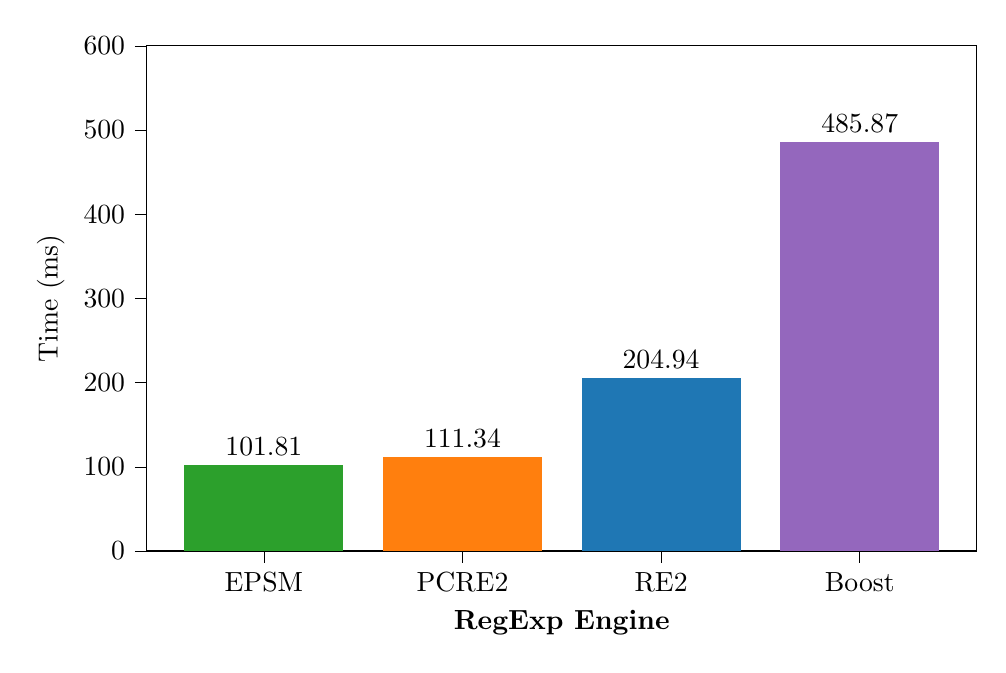
\begin{tikzpicture}
    \definecolor{crimson2143940}{RGB}{214,39,40}
    \definecolor{darkgray176}{RGB}{176,176,176}
    \definecolor{darkorange25512714}{RGB}{255,127,14}
    \definecolor{forestgreen4416044}{RGB}{44,160,44}
    \definecolor{lightgray204}{RGB}{204,204,204}
    \definecolor{mediumpurple148103189}{RGB}{148,103,189}
    \definecolor{sienna1408675}{RGB}{140,86,75}
    \definecolor{steelblue31119180}{RGB}{31,119,180}

\begin{axis}[
    width=\textwidth,
    height=8cm,
    tick align=outside,
    tick pos=left,
    x grid style={darkgray176},
    xlabel={\textbf{RegExp Engine}},
    xmin=-0.59, xmax=3.59,
    xtick style={color=black},
    xtick={0,1,2,3},
    xticklabels={EPSM, PCRE2, RE2, Boost},
    y grid style={darkgray176},
    ylabel={Time (ms)},
    ymin=0, ymax=600.172420926392,
    ytick style={color=black}
    ]
        
    \draw[draw=none,fill=forestgreen4416044] (axis cs:-0.4,0) rectangle (axis cs:0.4,101.814205093043);
    \draw[draw=none,fill=darkorange25512714] (axis cs:0.6,0) rectangle (axis cs:1.4,111.341547738347);
    \draw[draw=none,fill=steelblue31119180] (axis cs:1.6,0) rectangle (axis cs:2.4,204.944238894516);
    \draw[draw=none,fill=mediumpurple148103189] (axis cs:2.6,0) rectangle (axis cs:3.4,485.878496120373);
    \draw (axis cs:0,101.814205093043) ++(0pt,0pt) node[
      scale=1,
      anchor=south,
      text=black,
      rotate=0.0
    ]{101.81};
    \draw (axis cs:1,111.341547738347) ++(0pt,0pt) node[
      scale=1,
      anchor=south,
      text=black,
      rotate=0.0
    ]{111.34};
    \draw (axis cs:2,204.944238894516) ++(0pt,0pt) node[
      scale=1,
      anchor=south,
      text=black,
      rotate=0.0
    ]{204.94};
    \draw (axis cs:3,485.878496120373) ++(0pt,0pt) node[
      scale=1,
      anchor=south,
      text=black,
      rotate=0.0
    ]{485.87};
    \end{axis}
    \end{tikzpicture}
    \caption{Matching performance on TPC-H Q13. Time is the mean ($\mu$) of three runs of the benchmark. Our SIMD implementation based on EPSM algorithm is the fastest.}\label{fig:tpchres}
\end{figure}

Figure \ref{fig:tpchres} shows the benchmark results. The results show that our SIMD implementation based on the EPSM algorithm was the fastest engine. It achieved a speedup of $2x$ over the heavily optimized RE2. It was also slightly faster than PCRE2 with a speedup of $1.1x$. The engines (Ours, RE2, and PCRE2) were much faster than the baseline Boost achieving $4.8x$, $2.37x$, and $4.36x$ speedup, respectively.

The results from this benchmark show the potential performance gains of applying SIMD optimizations to simple patterns and literals. It opens the door for investigating the performance gains by adding these optimizations not only to literals but also for matching sub-patterns inside more complex ones, as discussed in the Future Work section \ref{futurework}.

\subsection{Regex-Redux Benchmark}\label{regexredux}
Regex-Redux \cite{regexredux} is a benchmark with nine simple patterns representing DNA 8-mers and their reverse and a dataset consisting of $90,000$ rows of DNA Sequences.

This benchmark aims to act as a baseline for performance analysis. The benchmark consists of simple patterns with alternations that the engines can optimize. It also has a relatively small number of rows, so we investigate the performance hit due to code-generation and compilation.

{\renewcommand{\arraystretch}{1.5}% for the vertical padding
\begin{table}[H]
\centering
\begin{adjustbox}{width=1.3\textwidth,center=\textwidth}
\begin{tabular}{|l|c|c|c|c|c|c|c|c|}
\hline
\diagbox{Pattern}{Engine} & RE2 & PCRE2 & LLVM U8 & LLVM U32 & CPP U8 & CPP U32 & Boost & \textbf{\# Matches} \\
\hline
agggtaaa|tttaccct & 12.94 & \bfseries 11.52 & 102.28 & 60.09 & 172.55 & 96.29 & 108.04 & 32 \\\hline
[cgt]gggtaaa|tttaccc[acg] & \bfseries 13.23 & 13.89 & 108.27 & 63.76 & 197.88 & 110.16 & 131.96 & 115 \\\hline
a[act]ggtaaa|tttacc[agt]t & \bfseries 12.81 & 13.88 & 111.40 & 65.38 & 197.96 & 107.51 & 117.59 & 368 \\\hline
agg[act]taaa|ttta[agt]cct & 13.15 & \bfseries 11.90 & 113.48 & 65.12 & 183.97 & 111.14 & 108.23 & 466 \\\hline
aggg[acg]aaa|ttt[cgt]ccct & 13.02 & \bfseries 12.13 & 127.64 & 77.61 & 198.36 & 148.26 & 108.55 & 135 \\\hline
agggtaa[cgt]|[acg]ttaccct & \bfseries 12.85 & 14.05 & 111.92 & 66.59 & 194.38 & 121.78 & 132.19 & 197 \\\hline
agggta[cgt]a|t[acg]taccct & \bfseries 13.12 & 13.91 & 117.44 & 66.17 & 207.59 & 113.27 & 118.19 & 139 \\\hline
agggt[cgt]aa|tt[acg]accct & \bfseries 12.83 & 13.41 & 116.55 & 67.72 & 181.65 & 115.40 & 110.70 & 137 \\\hline
ag[act]gtaaa|tttac[agt]ct & 12.93 & \bfseries 12.36 & 122.69 & 67.66 & 205.62 & 101.46 & 109.35 & 254 \\\hline
\end{tabular}
\end{adjustbox}
\caption{Performance Evaluation results on RegexDNA Benchmark. Time (in Milliseconds) is the mean ($\mu$) of five runs of the benchmark. Engines are configured to find partial matches (i.e, in any position of the text) for the patterns. Engines with better pattern optimizations are the fastest.}\label{tab:evalrgxdna}
\end{table}}

Table \ref{tab:evalrgxdna} shows the results for each pattern in the benchmark. RE2 and PCRE2 achieved the top performance while our implementation came at a distant third with a slowdown factor of $4x$.

The reasoning behind our slowdown is that these patterns can be optimized into string literals and searched using SIMD operations. PCRE2 does that \cite{pcre2opts} and that is why despite being JITed, it still has good performance. RE2 also uses SIMD and \texttt{\textbf{memchr(3)}} to skip ahead and match such patterns. Also, the number of matches for these patterns is too small (less than $0.2\%$), so optimized patterns can skip many characters. Our prototype implementation does not include such optimizations and thus achieved a worse performance and reads all the input text.

The results also show that our implementation using UTF-32 was faster than UTF-8 with a factor of $2x$. As both, the patterns and text do not include Unicode, the compilation time impact on UTF-32 is minimal, and at run-time, it has an overall smaller number of states that increase the matching speed.

This benchmark shows the effect of optimizations on regular expressions matching performance, especially with a low number of rows where there are not many performance gains from the compilation.

\subsection{Logs Benchmark}

LogHub \cite{loghub} maintains a collection of system logs, which are freely accessible for research purposes. Some logs are from prior studies' production data, while others are from genuine systems in their lab environment. The logs are not cleaned, anonymized, or altered in any manner.

In this benchmark, we used the \textit{Spark Logs} dataset from Loghub, which contains $33,236,604$ log messages from Spark jobs. Table \ref{tab:pattlogbench} shows the four patterns we applied to this dataset to evaluate the performance of the engines. It also shows what each pattern does and the number of expected matches for each pattern. It should be noted that the patterns may not be strictly correct or ideal. We simply require something to test the performance.

This benchmark aims to present a real scenario for our use case with tens of millions of rows and patterns that are not too complex but useful for analysis.

{\renewcommand{\arraystretch}{1.2}% for the vertical padding
\begin{table}[H]
\centering
% \begin{adjustbox}{width=1.2\textwidth,center=\textwidth}
\small
\makebox[\textwidth]{%
\begin{tabularx}{1.25\textwidth}{|l|X|l|l|}
\hline
\# & Pattern & Description & Matches\\
\hline
\rownumberthree & \texttt{\textbf{({[}a-zA-Z{]}{[}a-zA-Z0-9{]}*)://({[}\textasciicircum /\textvisiblespace{]}+)(/{[}\textasciicircum  \textvisiblespace{]}*)?}} & URI (protocol://server/path) & 793,701\\ \hline

\rownumberthree & \texttt{\textbf{{[}a-zA-Z0-9\_.+-{]}+@{[}a-zA-Z0-9-{]}+{[}.{]}{[}a-zA-Z0-9-.{]}+}} & Email &  15,002\\ \hline

\rownumberthree & \texttt{\textbf{({[}0-9{]}{[}0-9{]}?)/({[}0-9{]}{[}0-9{]}?)/({[}0-9{]}{[}0-9{]}({[}0-9{]}{[}0-9{]})?)}} & Date (day/month/year) & 27,410,266\\ \hline

\rownumberthree & \texttt{\textbf{({[}a-zA-Z{]}{[}a-zA-Z0-9{]}*)://({[}\textasciicircum /\textvisiblespace{]}+)(/{[}\textasciicircum \textvisiblespace{]}*)?|{[}a-zA-Z0-9\_.+-{]}+@{[}a-zA-Z0-9-{]}+{[}.{]}{[}a-zA-Z0-9-.{]}+}} & URI or Email & 793,802\\
\hline
\end{tabularx}}
% \end{adjustbox}
\caption{Patterns used in the Log benchmark and number of matches.}\label{tab:pattlogbench}
\end{table}
}

Table \ref{tab:evallogbench} shows the benchmark results for each pattern and engine under test. Boost was the worst-performing engine by a factor of $20x-40x$ compared to the other engines, so we exclude it from the analysis as it struggles with large data sets and is unsuitable for our use case. Figure \ref{fig:graphlogbench} shows the results after excluding Boost Engine.

{\renewcommand{\arraystretch}{1.6}% for the vertical padding
\begin{table}[H]
\centering
\begin{adjustbox}{width=1.2\textwidth,center=\textwidth}
\large
\begin{tabular}{|l|l|l|l|l|l|l|l|l|}
\hline
\diagbox{Pattern}{Engine} & RE2 & PCRE2 & DFA LLVM U8 & DFA LLVM U32 & DFA CPP U8 & DFA CPP U32 & Boost\\
\hline
URI (protocol://server/path) & 6.76 & \bfseries 2.67 & 6.31 & 9.57 & 6.71 & 9.16 & 105.27\\ \hline
Email & 6.84 & \bfseries 5.56 & 6.29 & 9.74 & 6.52 & 9.83 & 102.95\\ \hline
Date (day/month/year) & 3.21 & 2.40 & \bfseries 1.78 & 2.28 & 1.83 & 2.15 & 34.53 \\ \hline
URI or Email & 6.73 & 16.86 & \bfseries 6.15 & 10.12 & 6.15 & 9.75 & 192.92\\ \hline
\end{tabular}
\end{adjustbox}
\caption{Performance Evaluation results on Logs Benchmark. Time (in seconds) is the mean ($\mu$) of three runs of the benchmark. Engines are configured to find partial matches (i.e, in any position of the text) for the patterns. JIT engines are the fastest.}\label{tab:evallogbench}
\end{table}
}

The first pattern matches URIs. $2.37\%$ of the rows match this pattern. The best performing engine was PCRE2, beating our LLVM UTF-8 implementation (second-best engine) by a speedup factor of $2.36x$. Still, both engines were faster than the optimized but interpreted RE2. The results show that JIT compilation was beneficial, and the compilation time was amortized over a large number of times the matching function was used.

The second pattern matches Emails. Less than $0.004\%$ of the rows match this pattern. PCRE2 was once again the fastest engine but by a smaller factor of $1.13x$ than the second-best engine (LLVM UTF-8). They both, once again, were faster than RE2. The much smaller number of matches can explain the drop in performance for PCRE2; therefore, much time was spent navigating the text, and SIMD optimizations can not be utilized here.

The third pattern matches Dates. Every log line starts with the date; therefore, $82.4\%$ of the rows (since a log can span multiple lines) match this pattern. Our Implementation was the fastest on this, with a speedup factor of $1.34x$ over the second-best engine, PCRE2. This speedup in our engine is due to our early termination, where we do not process the line once a match was found and report success immediately, and far less time is spent navigating the input text.

The fourth and last pattern alternates the first and second pattern and matches either a URI or an email. $2.38\%$ of the rows match this pattern. The performance of PCRE2 suddenly dropped on this pattern, and the best performing was our implementation, followed by RE2. The performance drop for PCRE2 can be attributed to the fact that PCRE2 uses a backtracking algorithm which usually struggles with complex alternations since it has to try all candidates.

\begin{figure}[H]
    \centering
    \hspace*{-45pt}
    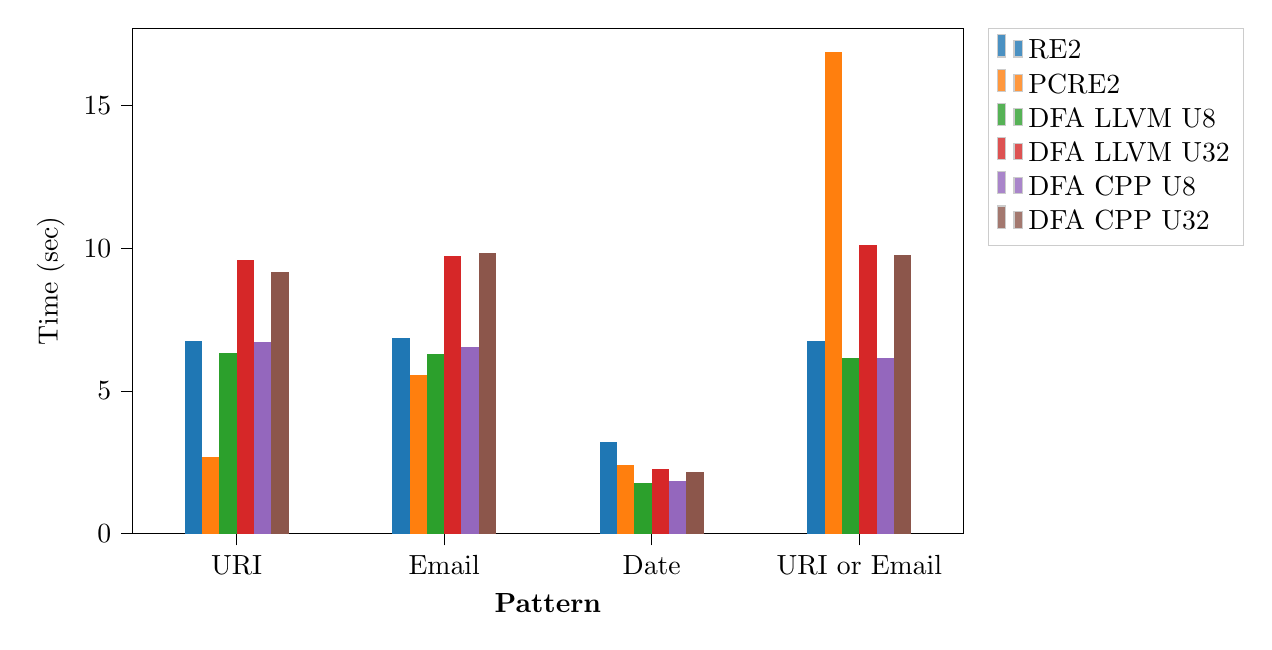
\begin{tikzpicture}
    \definecolor{crimson2143940}{RGB}{214,39,40}
    \definecolor{darkgray176}{RGB}{176,176,176}
    \definecolor{darkorange25512714}{RGB}{255,127,14}
    \definecolor{forestgreen4416044}{RGB}{44,160,44}
    \definecolor{lightgray204}{RGB}{204,204,204}
    \definecolor{mediumpurple148103189}{RGB}{148,103,189}
    \definecolor{sienna1408675}{RGB}{140,86,75}
    \definecolor{steelblue31119180}{RGB}{31,119,180}
    
    \begin{axis}[
    legend cell align={left},
    legend style={
      fill opacity=0.8,
      draw opacity=1,
      text opacity=1,
    %   at={(0.03,0.97)},
        % at={(-0.5,-0.5)},
      anchor=north west,
      legend pos= outer north east,
      draw=lightgray204,
    },
    % scale axis only,
    bar width=9pt,
    width=\textwidth,
    height=8cm,
    tick align=outside,
    tick pos=left,
    x grid style={darkgray176},
    xlabel={\textbf{Pattern}},
    xmin=-0.5, xmax=3.5,
    xtick style={color=black},
    xtick={0,1,2,3},
    xticklabel style={rotate=0},
    xticklabels={URI,Email,Date,URI or Email},
    y grid style={darkgray176},
    ymin=0, ymax=17.7023160803132,
    ytick style={color=black},
    ylabel={Time (sec)}
    ]
    \draw[draw=none,fill=steelblue31119180] (axis cs:-0.25,0) rectangle (axis cs:-0.166666666666667,6.75804211944342);
    \addlegendimage{ybar,ybar legend,draw=none,fill=steelblue31119180}
    \addlegendentry{RE2}
    
    \draw[draw=none,fill=steelblue31119180] (axis cs:0.75,0) rectangle (axis cs:0.833333333333333,6.83566853404045);
    \draw[draw=none,fill=steelblue31119180] (axis cs:1.75,0) rectangle (axis cs:1.83333333333333,3.20648544281721);
    \draw[draw=none,fill=steelblue31119180] (axis cs:2.75,0) rectangle (axis cs:2.83333333333333,6.73386627311508);
    \draw[draw=none,fill=darkorange25512714] (axis cs:-0.166666666666667,0) rectangle (axis cs:-0.0833333333333333,2.66720288681487);
    \addlegendimage{ybar,ybar legend,draw=none,fill=darkorange25512714}
    \addlegendentry{PCRE2}
    
    \draw[draw=none,fill=darkorange25512714] (axis cs:0.833333333333333,0) rectangle (axis cs:0.916666666666667,5.56027145497501);
    \draw[draw=none,fill=darkorange25512714] (axis cs:1.83333333333333,0) rectangle (axis cs:1.91666666666667,2.39978482263784);
    \draw[draw=none,fill=darkorange25512714] (axis cs:2.83333333333333,0) rectangle (axis cs:2.91666666666667,16.8593486479173);
    \draw[draw=none,fill=forestgreen4416044] (axis cs:-0.0833333333333333,0) rectangle (axis cs:-1.38777878078145e-17,6.309387218828);
    \addlegendimage{ybar,ybar legend,draw=none,fill=forestgreen4416044}
    \addlegendentry{DFA LLVM U8}
    
    \draw[draw=none,fill=forestgreen4416044] (axis cs:0.916666666666667,0) rectangle (axis cs:1,6.2886191084981);
    \draw[draw=none,fill=forestgreen4416044] (axis cs:1.91666666666667,0) rectangle (axis cs:2,1.78335128538311);
    \draw[draw=none,fill=forestgreen4416044] (axis cs:2.91666666666667,0) rectangle (axis cs:3,6.15050168645879);
    \draw[draw=none,fill=crimson2143940] (axis cs:-3.46944695195361e-17,0) rectangle (axis cs:0.0833333333333333,9.57483077421784);
    \addlegendimage{ybar,ybar legend,draw=none,fill=crimson2143940}
    \addlegendentry{DFA LLVM U32}
    
    \draw[draw=none,fill=crimson2143940] (axis cs:1,0) rectangle (axis cs:1.08333333333333,9.73707360339661);
    \draw[draw=none,fill=crimson2143940] (axis cs:2,0) rectangle (axis cs:2.08333333333333,2.27664395173391);
    \draw[draw=none,fill=crimson2143940] (axis cs:3,0) rectangle (axis cs:3.08333333333333,10.1164847991119);
    \draw[draw=none,fill=mediumpurple148103189] (axis cs:0.0833333333333333,0) rectangle (axis cs:0.166666666666667,6.71010144116978);
    \addlegendimage{ybar,ybar legend,draw=none,fill=mediumpurple148103189}
    \addlegendentry{DFA CPP U8}
    
    \draw[draw=none,fill=mediumpurple148103189] (axis cs:1.08333333333333,0) rectangle (axis cs:1.16666666666667,6.51985231352349);
    \draw[draw=none,fill=mediumpurple148103189] (axis cs:2.08333333333333,0) rectangle (axis cs:2.16666666666667,1.82853213883936);
    \draw[draw=none,fill=mediumpurple148103189] (axis cs:3.08333333333333,0) rectangle (axis cs:3.16666666666667,6.15106135172149);
    \draw[draw=none,fill=sienna1408675] (axis cs:0.166666666666667,0) rectangle (axis cs:0.25,9.15627114661038);
    \addlegendimage{ybar,ybar legend,draw=none,fill=sienna1408675}
    \addlegendentry{DFA CPP U32}
    
    \draw[draw=none,fill=sienna1408675] (axis cs:1.16666666666667,0) rectangle (axis cs:1.25,9.83319650404155);
    \draw[draw=none,fill=sienna1408675] (axis cs:2.16666666666667,0) rectangle (axis cs:2.25,2.15193498693407);
    \draw[draw=none,fill=sienna1408675] (axis cs:3.16666666666667,0) rectangle (axis cs:3.25,9.74742509176334);
    \end{axis}
    
    \end{tikzpicture}
    \caption{Performance Evaluation results on Logs Benchmark without Boost Engine.}\label{fig:graphlogbench}
\end{figure}

Overall, the results on this benchmark show that adding JIT compiling to even a less optimized engine can be faster than a heavily optimized but interpreted engine. When the number of rows to process is large, the cost of compilation is amortized over the large number of runs required.